\subsection{\color{ForestGreen}Properties of CFL's, CYK}
 Many questions that can be decided for regular languages cannot be decided for CFLs. E.g. "are two CFL's the same?", "are two CFL's disjoint?"
\subsubsection{Decision Properties}
\textbf{Emptiness Problem}: 
\begin{itemize}
    \item Eliminate variables that generate no terminal string. 
    \item If the start symbol is one of these, then the CFL is empty, o.w. no.
\end{itemize}
\textbf{Membership Problem}: "Is string $w$ in $L(G)$?"
\begin{itemize}
    \item If $w = \epsilon$, test that the start symbol is nullable.
    \item Otherwise, assume $G$ is in CNF and run \textbf{CYK}.
\end{itemize}

\begin{Figure}
 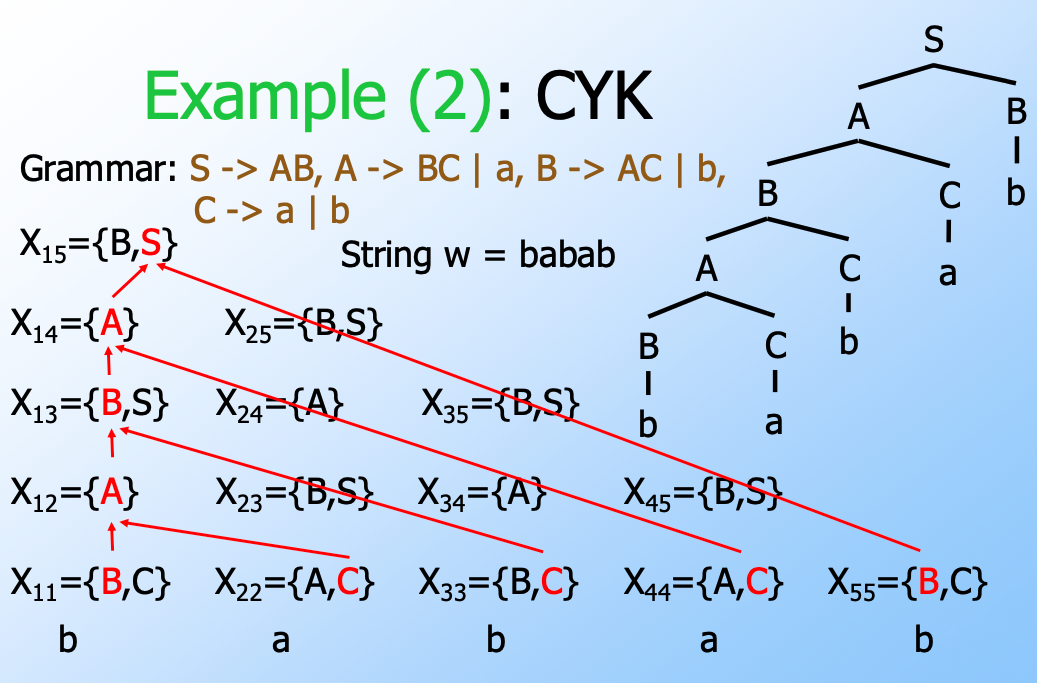
\includegraphics[width=0.7\linewidth]{figures/CYK.png}
\end{Figure}
\textbf{Infiniteness Problem}:
\begin{itemize}
    \item Use the pumping lemma constant $n$. 
    \item If there is a string in the language of length between $n$ and $2n -1$, then the language is infinite, otherwise not.
\end{itemize}
\subsubsection{Closure Properties}
Let $L$ and $M$ be CFL's with grammars $G$ and $H$ with no variables in common.
Let $S_1$ and $S_2$ be the start symbols of $G$ and $H$. 

\textbf{Union}: Form a new grammar for $L\cup M$.
\begin{itemize}
    \item Combine all the symbols and productions of $G$ and $H$. 
    \item Add a new start symbol $S$. 
    \item Add productions $S \rightarrow S_1 | S_2 $.
\end{itemize}
\textbf{Concatenation}: Form a new grammar for $LM$.
\begin{itemize}
    \item Add a new start symbol $S$.
    \item Add productions $S \rightarrow S_1S_2$. 
    \item Every derivation from $S$ results in a string in $L$ followed by one in $M$.
\end{itemize}
\textbf{Star}: Form a new grammar for $L^*.$
\begin{itemize}
    \item Introduce a new start symbol $S$ and the productions $S \rightarrow S_1 S | \epsilon.$
    \item A rightmost derivation from $S$ generates a sequence of zero or more $S_1$’s, each of which generates some string in $L$.
\end{itemize}
\textbf{Reversal}: Form a new grammar for $L^R$.
\begin{itemize}
    \item Let $G$ have $S \rightarrow 0S1 | 01$.
\item The reversal of $L(G)$ has grammar $S\rightarrow 1S0 | 10.$
\end{itemize}
\textbf{Homomorphism}: Construct a grammar for $h(L)$.
\begin{itemize}
    \item Let $h$ be a homomorphism on the terminal symbols of $G$.
    \item  Replace each terminal symbol $a$ by $h(a)$.
\end{itemize}
\textbf{Inverse Homomorphism}:  $L = L(P)$ for some PDA $P$, we construct PDA $P^\prime$ to accept $h^{-1}(L)$.

$\mathbf{P^\prime}$: States are pairs $[q, b]$, where $q$ is a state of $P$, $b$ is a suffix of $h(a)$ for some symbol $a$. Thus, only a finite number of possible values
for $b$. Stack symbols of $P^\prime$ are those of $P$. Start state of $P^\prime$ is $[q_0 ,\epsilon ]$. Input symbols of $P^\prime$ are the symbols to which $h$ applies.
Final states of $P^\prime$ are the states $[q, \epsilon]$ such that $q$ is a final state of $P$.
Transitions of $P^\prime$: 
\begin{enumerate}
\item $\delta^\prime([q, \epsilon], a, X) = \{([q, h(a)], X)\}$ for
any input symbol $a$ of $P^\prime$ and any stack
symbol $X$.
\item $\delta^\prime ([q, bw], \epsilon, X)$ contains $([p, w], \alpha)$ if
$\delta (q, b, X)$ contains $(p, \alpha)$, where $b$ is
either an input symbol of $P$ or $\epsilon$. 
\end{enumerate}
\textbf{Intersection with a Regular Language}: run a DFA in parallel
with a PDA, and notice that the combination is a PDA. Thus the intersection of a CFL with a regular language is always a CFL.
\subsubsection{Nonclosure Properties}
\begin{itemize}
    \item CFL's are not closed under intersection. 
    \item CFL's are not closed under difference. Because any class of languages that is closed under difference must also be closed under intersection. 
\end{itemize}
